\chapter{Religion, Authority, and Education II}

This chapter follows J. Krishnamurti's second San Diego conversation with Dr. Alan W. Anderson on religion, authority, and education. There are no blackboard equations or validated visual diagrams for this lecture; the structure is therefore conceptual rather than computational. Still, the argument has a precise spine. Krishnamurti begins at the point where inquiry trembles and withdraws, traces that hesitation to education in function and measure, distinguishes freedom from authority, and ends by opening the next question: meditation as inseparable from religion, conduct, relationship, love, death, and care.

\section{The Brink Of Inquiry}

Anderson begins by returning to the previous conversation. The point at issue is not a doctrine but a threshold. In self-examination one comes to a brink: there is fear, trembling, hesitation, and then a withdrawal. Krishnamurti accepts the formulation and gives it its sharpest form: why do we not take the plunge? Why do we come to the edge and run away?

The lecture should be read from that question. The problem is not first whether one has the right belief about religion. The problem is whether the mind can stay with inquiry when inquiry ceases to be comfortable.

\begin{align}
\hbox{inquiry} &\longrightarrow \hbox{brink} \longrightarrow \hbox{fear and trembling},\\
\hbox{fear and trembling} &\longrightarrow \hbox{withdrawal or flight}.
\end{align}

This is not a mathematical equation in the ordinary sense. It is a compact map of the spoken movement. Krishnamurti's question is whether the second line is inevitable.

\subsection{Question \& Answer}

\paragraph{Question.}
Why do we come to the brink of inquiry and not take the plunge?

\paragraph{Answer.}
Krishnamurti's first answer is that we have been educated for function rather than intelligence. We know how to function as engineers, professors, doctors, specialists, and members of a society that demands measurable competence. But the inquiry into religion, freedom, attention, and truth is not measurable in that way. When the mind trained by measure enters a field where there is no measure, it becomes uncertain; and when it is uncertain, it seeks dependence.

\begin{align}
\hbox{functional training}
&\longrightarrow \hbox{measure}
\longrightarrow \hbox{status}
\longrightarrow \hbox{dependence}
\longrightarrow \hbox{authority}.
\end{align}

The answer is therefore not simply that human beings are cowardly. The hesitation is bound up with education, social structure, and the mind's habit of looking for a measure before it will act.

\section{Function, Measure, And Status}

Krishnamurti does not reject function. Functional knowledge has its proper place. One must know how to build, heal, teach, calculate, repair, and communicate. The trouble begins when the structure of function becomes the model for the whole of life.

\begin{definition}
In this chapter, \emph{function} means the trained capacity to operate in a field of knowledge: a profession, a technique, a career, or a socially measurable skill.
\end{definition}

The point is delicate. In the field of function, one can measure performance. One can ask whether a bridge stands, whether a calculation is correct, whether a physician has diagnosed well, whether a student has mastered a procedure. But Krishnamurti says that when the mind turns to religion in the serious sense, it does not know what the measure is. And precisely there it begins to depend.

\begin{proposition}
When a mind trained chiefly by measurable function enters an immeasurable field, it tends to substitute authority for inquiry.
\end{proposition}

\begin{proof}
The argument follows the lecture's order.
\begin{enumerate}
\item Education emphasizes function, career, technique, and status.
\item Function is measured by external standards of success.
\item Religious inquiry, as Krishnamurti uses the phrase, has no such external measure.
\item The mind trained to rely on measure finds itself without its familiar instrument.
\item In that uncertainty it turns to those who claim to know.
\item The claim of another to know becomes authority.
\end{enumerate}
Thus dependence is not accidental; it is the carryover of one field into another.
\end{proof}

The contrast can be kept in a small table.

\begin{table}
\centering
\begin{tabular}{p{0.43\linewidth} p{0.43\linewidth}}
Field of knowledge & Field of inquiry \\
\hline
Function, technique, skill & Freedom, attention, direct seeing \\
Measure and comparison & No external measure \\
Instruction has a place & Authority obstructs inquiry \\
Thought is necessary & Thought must know its limit \\
\end{tabular}
\end{table}

\section{Freedom Before Inquiry}

The next movement of the lecture turns from education to perception. Krishnamurti says that to inquire there must be freedom first. Not freedom as a reward, not freedom at the end of obedience, but freedom at the beginning. If I inquire with a prejudice, I cannot inquire. If I inquire with a conclusion, I cannot inquire. If I look through an image, I do not see what is living.

The image is one of the important distinctions in this lecture. I may look at a tree through the screen of knowledge, at another person through memory, at nature through translation and enjoyment, or at religion through books and priests. In each case the living thing is replaced by a dead image.

\begin{align}
\hbox{living thing}
&\longrightarrow \hbox{image, memory, knowledge, translation}\\
&\longrightarrow \hbox{indirect perception}.
\end{align}

Krishnamurti is not asking for ignorance in the ordinary sense. He is distinguishing between knowledge as a useful function and knowledge as a screen. The same distinction will later return as the difference between thought in the field of knowledge and thought trying to construct reality.

\subsection{Question \& Answer}

\paragraph{Question.}
Can freedom and authority coexist in religious inquiry?

\paragraph{Answer.}
No. In the lecture's sequence, freedom and authority cannot possibly exist together. Authority may have a limited place in learning a technical function, but when the mind inquires into religion, God, truth, beauty, or freedom, authority becomes dependence. Krishnamurti's formulation is stronger still: freedom and intelligence go together, and intelligence has its own discipline, not the discipline of suppression or imitation, but the discipline of learning all the time.

Anderson then gives Krishnamurti the transition: this intelligence is immediate, not gradual. Krishnamurti accepts it. Perception is intelligence, and therefore perception is action.

\begin{align}
\hbox{freedom} &\longrightarrow \hbox{inquiry},\\
\hbox{attention} &\longrightarrow \hbox{intelligence},\\
\hbox{perception} &\longrightarrow \hbox{action}.
\end{align}

These arrows must be read carefully. They are not a doctrine to be memorized. Anderson himself notes that when this living movement is translated into a concept, it can again become a source of terror. Krishnamurti agrees: then it is no longer the thing itself.

\section{The Book, The Class, And The Clean Eye}

The middle of the conversation moves into Anderson's classroom. How is a teacher to handle inherited texts, scriptures, classical materials, and accumulated knowledge without making students second-hand? The question is practical, not decorative. It asks whether education can use books without installing authority at the center.

Krishnamurti answers by reversing the order. If he had a class, he says, he would not begin with the book. He would begin with freedom. The student is second-hand; do not pretend otherwise. The reality, if it is real, is original; therefore the mind that approaches it must be original, which means free.

The classroom sequence can be represented as a cautious editorial diagram.

\begin{figure}
\centering
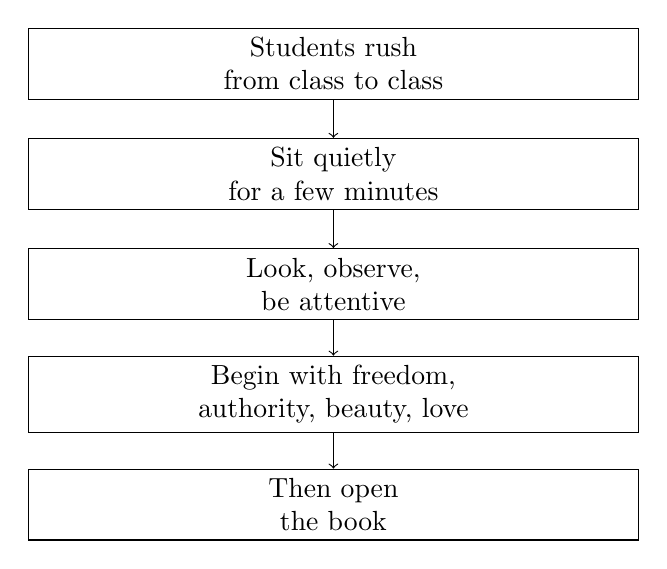
\begin{tikzpicture}
\node[draw, text width=0.62\linewidth, align=center] (a) at (0,0) {Students rush\\from class to class};
\node[draw, text width=0.62\linewidth, align=center] (b) at (0,-1.4) {Sit quietly\\for a few minutes};
\node[draw, text width=0.62\linewidth, align=center] (c) at (0,-2.8) {Look, observe,\\be attentive};
\node[draw, text width=0.62\linewidth, align=center] (d) at (0,-4.2) {Begin with freedom,\\authority, beauty, love};
\node[draw, text width=0.62\linewidth, align=center] (e) at (0,-5.6) {Then open\\the book};
\draw[->] (a) -- (b);
\draw[->] (b) -- (c);
\draw[->] (c) -- (d);
\draw[->] (d) -- (e);
\end{tikzpicture}
\caption{A transcript-based reconstruction of Krishnamurti's classroom order: quiet attention before the book.}
\end{figure}

\subsection{Question \& Answer}

\paragraph{Question.}
How can a book be read without becoming second-hand?

\paragraph{Answer.}
The book must not come first. If the student begins with the book as authority, the student accumulates what others have said. If the student begins with freedom, quietness, observation, and self-knowing, then the book can be read with what Anderson calls a clean eye. The book is still there, but it has lost its power to replace direct inquiry.

\begin{align}
\hbox{quiet attention}
\longrightarrow \hbox{self-knowing}
\longrightarrow \hbox{book read with a clean eye}.
\end{align}

Krishnamurti then gives the stronger version: the real book is oneself. If one can read that book, one has learned what is essential, except for functional knowledge.

\section{The Original Mind And The Real Book}

The phrase ``second-hand'' is central to this part of the conversation. The mind that merely repeats what the priest, scripture, guru, philosopher, or teacher has said is not original. But Krishnamurti does not mean originality as novelty, self-expression, or artistic cleverness. He means a free mind.

\begin{definition}
An \emph{original mind}, in this lecture, is not a mind producing new opinions. It is a mind free enough to look, observe, and learn without dependence on spiritual authority.
\end{definition}

This brings the inquiry back to religion. Can the mind put away everything that man has talked about, invented, imagined, or believed about religion and God? Can consciousness empty itself of what has been said about reality? Krishnamurti insists that otherwise we do not discover. We merely repeat.

Here the chapter must preserve the rhythm of the repeated question. He asks it once as freedom from authority. He asks it again as freedom from inherited religious structure. He asks it again as whether the mind, heart, and brain can be free of what man has said about reality.

\begin{align}
\hbox{borrowed claim} &\longrightarrow \hbox{belief},\\
\hbox{belief} &\longrightarrow \hbox{repetition},\\
\hbox{repetition} &\longrightarrow \hbox{no discovery}.
\end{align}

This is the lecture's negative discipline. To put away authority is not to become careless. It is to stop pretending that repetition is discovery.

\section{Leaving The World, Carrying The Baggage}

Krishnamurti then tells the Kashmir story. A group of monks comes to him from the mountains. They speak of people who have left the world. Krishnamurti asks what that means. If they have left the world, have they left the memory of the world? Have they left the knowledge put together by gurus, teachers, books, sacrifice, torture, and renunciation?

Anderson gives the image: they went up the mountain with all this baggage. Krishnamurti accepts it. The world they put away outwardly is still being carried inwardly.

\begin{figure}
\centering
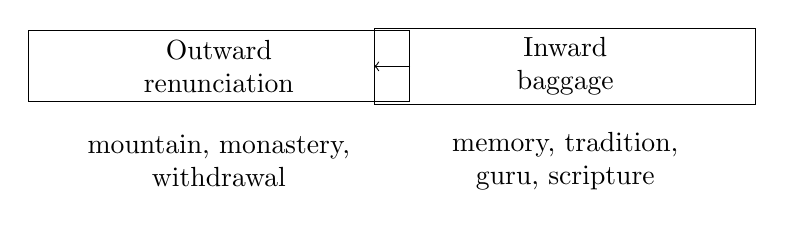
\begin{tikzpicture}
\node[draw, text width=0.38\linewidth, align=center] (left) at (-2.2,0) {Outward\\renunciation};
\node[draw, text width=0.38\linewidth, align=center] (right) at (2.2,0) {Inward\\baggage};
\node[text width=0.38\linewidth, align=center] (l2) at (-2.2,-1.2) {mountain, monastery,\\withdrawal};
\node[text width=0.38\linewidth, align=center] (r2) at (2.2,-1.2) {memory, tradition,\\guru, scripture};
\draw[->] (left) -- (right);
\end{tikzpicture}
\caption{Outward withdrawal does not itself free the mind from accumulated memory and authority.}
\end{figure}

This story prepares the late distinction between aloneness and isolation. Isolation can be manufactured by withdrawal, walls, practices, and separations. Aloneness, as Krishnamurti uses the word, comes only when the mind puts away the things of thought.

\section{Aloneness, Falsehood, And Meditation}

Krishnamurti asks whether the mind can be completely alone: not isolated, not withdrawn, not enclosed by a wall, but alone because the accretions of thought have ended. He then gives the clearest statement of thought's limit in the lecture. Thought is the response of memory, knowledge, and experience stored in the brain. Therefore thought is of the past. It may function in the field of knowledge, but not in the other field.

\begin{align}
\hbox{memory} + \hbox{knowledge} + \hbox{experience}
&\longrightarrow \hbox{thought},\\
\hbox{thought} &\longrightarrow \hbox{the past},\\
\hbox{thought of time} &\not\longrightarrow \hbox{the timeless}.
\end{align}

The last line is a schematic, not a physical theorem. It preserves Krishnamurti's spoken claim that thought, being of time, cannot create what has no time.

The next move is important. Krishnamurti does not ask for bravery, sacrifice, or torture. He asks for perception of the false. To see the false is already to see truth in the false; and to see what is commonly taken as truth as false is to strip the mind of inward deception.

Desire then enters the argument. The desire to experience, to achieve, to arrive, even to be enlightened, creates illusion. The mind must therefore be free of the pursuit of desire and fulfilment. This recalls earlier conversations on fear, desire, and pleasure, but here the point is placed inside the inquiry into religion.

\begin{align}
\hbox{desire to experience}
&\longrightarrow \hbox{projection},\\
\hbox{projection}
&\longrightarrow \hbox{illusion}.
\end{align}

Anderson notices a danger: one may repeat these questions and think one has grasped them. Krishnamurti answers: one has grasped the words. This is a crucial caution for the chapter itself. The structure can be mapped, but the map is not the movement.

The conversation then turns toward meditation. Krishnamurti says that religion, in the sense under discussion, and meditation go together. Religion is not an idea. It is actual conduct in daily life: thought, speech, behavior, relationship, love, death, and care. Anderson brings in the root sense of meditation as thinking, pondering, going into, and caring for; Krishnamurti sharpens the point from carefulness to caring.

\begin{align}
\hbox{conduct} + \hbox{relationship} + \hbox{love} + \hbox{death} + \hbox{care}
\longrightarrow \hbox{religion and meditation}.
\end{align}

The lecture ends not with a completed theory of meditation, but with a threshold. Meditation will have to be explored within the whole field of authority, fear, desire, social pressure, and religious degeneration that the conversation has just unfolded.

\section{Summary}

This conversation begins with hesitation at the brink and ends at the threshold of meditation. Its order matters. First, Krishnamurti asks why we withdraw when inquiry becomes serious. Then he traces the withdrawal to education in function, measure, status, and dependence. He distinguishes freedom from authority and direct seeing from the image. He brings the question into the classroom, where books can either reinforce second-hand living or be read with a clean eye. He then deepens the inquiry through the demand for an original mind, the image of the real book as oneself, and the Kashmir story of outward renunciation carrying inward baggage.

The final movement is the most exacting. Aloneness is not isolation. Thought has its place in knowledge but cannot govern the inquiry into the timeless. Desire to achieve spiritual experience creates illusion. Religion is not belief or institution but the regeneration of life through attention, conduct, relationship, love, death, and care. Meditation is therefore not an escape from daily life; it is the next question opened by the whole conversation.